\documentclass{scrartcl}

\usepackage{amssymb}
\usepackage{amsmath}
\usepackage{tikz}
\usetikzlibrary{arrows, arrows.meta}

%from Badiou - Conditions, pp. 121 + 197
%based on the more polished versions in Mullarkey - Post-Continental Philosophy, ch. 5

\begin{document}
%\tikzset{->-/.style={decoration={
%			markings,
%			mark=at position #1 with {\arrow{>}}},postaction={decorate}}}
	
	%\begin{figure}
	%	\centering
	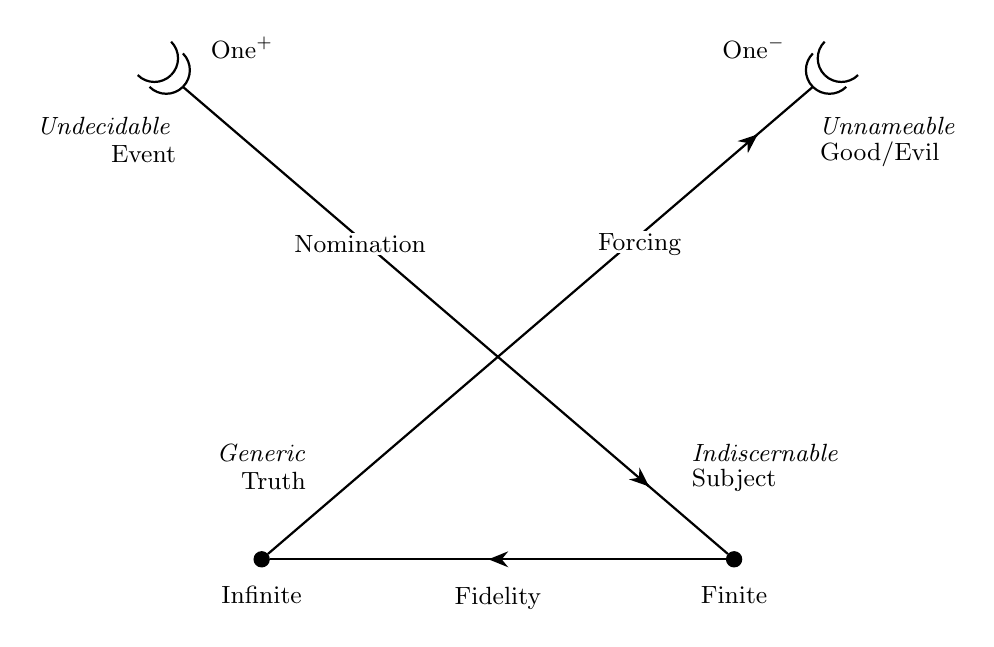
\begin{tikzpicture}
	\node[circle,draw=black, fill=black, inner sep=0pt,minimum size=5.5pt] (l) at (-3,0) {};
	\node[circle,draw=black, fill=black, inner sep=0pt,minimum size=5.5pt] (r) at (3,0) {};
	\coordinate (L) at (-4,6);
	\coordinate (R) at (4,6);
	
	%arrows
	\draw[thick] (r)--(l);		%[->-=0.52,thick]
	\draw[thick] (L)--(r);		%[->-=0.85,thick]
	\draw[thick] (l)--(R);		%[->-=0.90,thick]
	
	%labels	
	\node at (-3.25,6.5) {{\small One$^+$}};
	\node at  (3.25,6.5) {{\small One$^-$}};
	%
	\node at (-5,5.5)	 {{\small \textit{Undecidable}}};
	\node at (-4.5,5.15) {{\small Event}};
	\node at (4.95,5.5)  {{\small \textit{Unnameable}}};
	\node at (4.85,5.15) {{\small Good/Evil}};
	%
	\draw[line width=8pt, color=white] (-3,4)--(-1,4);		%manual fill
	\node at (-1.75,4) {{\small Nomination}};
	\draw[line width=8pt, color=white] (1,4.03)--(3,4.03);	%manual fill
	\node at (1.8,4) {{\small Forcing}};
	%
	%optional - diagonal labels
	%\node at (-1.75,4.4) {\rotatebox{320}{{\small Nomination}}};
	%\node at (2,4.55) {\rotatebox{40}{{\small Forcing}}};
	%
	\node at (-3,1.35) {{\small \textit{Generic}}};
	\node at (-2.85,1) {{\small Truth}};
	\node at (3.4,1.35){{\small \textit{Indiscernable}}};
	\node at (3,1.00)  {{\small Subject}};
	%
	\node at (-3,-.45) {{\small Infinite}};
	\node at (0,-0.5)  {{\small Fidelity}};
	\node at (3,-0.45) {{\small Finite}};
	
	%arcs
	\draw[thick] (R) arc (225:315:3mm);	 %right arcs: lower arc, left part
	\draw[thick] (R) arc (225:135:3mm);	 %lower arc, right part
	%
	\draw[thick] (4.15,6.15) arc (225:315:3mm);	 %right arcs: upper arc, left part
	\draw[thick] (4.15,6.15) arc (225:135:3mm);	 %upper arc, right part
	%
	\draw[thick] (L) arc (315:225:3mm);	 %left arcs: lower arc, left part
	\draw[thick] (L) arc (315:405:3mm);	 %lower arc, right part
	%
	\draw[thick] (-4.15,6.15) arc (315:225:3mm);  %left arcs: upper arc, left part
	\draw[thick] (-4.15,6.15) arc (315:405:3mm);  %upper arc, right part
	
	%arrowheads
	%I have to add the arrowheads manually, since I can't readjust both size & position
	\draw[-{Stealth[length=2.5mm,width=2mm]}, thick] (0,0)--(-0.12,0);
	\draw[-{Stealth[length=2.5mm,width=2mm]}, thick] (3.29,5.388)--(3.3,5.3965);
	\draw[-{Stealth[length=2.5mm,width=2mm]}, thick] (1.9143,0.93)--(1.92,0.925);
	
	%\draw[help lines] (-5,-1) grid (5,7);
	\end{tikzpicture}
	%	\caption{...}
	%\end{figure}
	
	
	\vspace{2cm}
	
	
	%NB: `H' stands for `humanity function'
	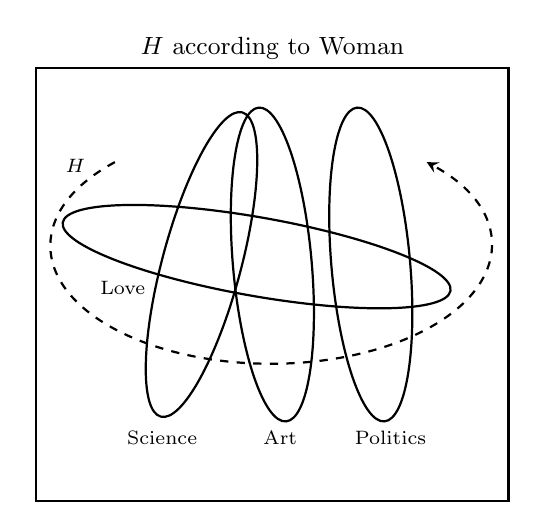
\begin{tikzpicture}[>=stealth]
	\draw[thick] (0,0) rectangle (6,5.5);
	\draw[->,dashed,thick] (1,4.3) arc (135:405:2.8cm and 1.5cm);
	
	%ellipses
	\draw[thick] (2.8,3.1)circle [x radius=2.5cm, y radius=0.5cm, rotate=170];	%horizontal ellipsis
	\draw[thick] (2.1,3)  circle [x radius=2cm, y radius=0.5cm, rotate=75];	%left vertical ellipsis
	\draw[thick] (3,3)    circle [x radius=2cm, y radius=0.5cm, rotate=95];	%middle vertical ellipsis
	\draw[thick] (4.25,3) circle [x radius=2cm, y radius=0.5cm, rotate=95];	%right vertical ellipsis
	
	%labels
	\node at (3,5.75) 	{{\small $H$ according to Woman}};
	\node at (0.5,4.25)	{{\scriptsize $H$}};
	\node at (1.1,2.7) 	{{\scriptsize Love}};
	\node at (1.6,0.8) 	{{\scriptsize Science}};
	\node at (3.1,0.8) 	{{\scriptsize Art}};
	\node at (4.5,0.8) 	{{\scriptsize Politics}};
	%\draw[help lines] (0,0) grid (6,6);
	\end{tikzpicture}
	%
	%
	\hspace{0.5cm}
	%
	%
	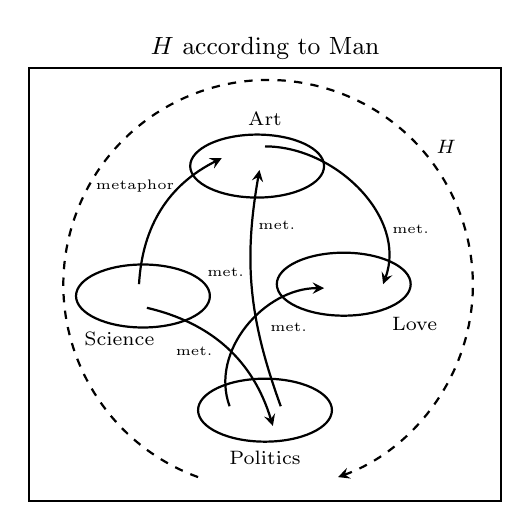
\begin{tikzpicture}[>=stealth]
	\draw[thick] (0,0) rectangle (6,5.5);
	\draw[->,dashed,thick] (2.15,0.3) arc (250:-70:2.6cm);
	
	%ellipses
	\draw[thick] (2.9,4.25) circle [x radius=0.85cm, y radius=0.4cm];
	\draw[thick] (1.45,2.6) circle [x radius=0.85cm, y radius=0.4cm];
	\draw[thick] (4,2.75)   circle [x radius=0.85cm, y radius=0.4cm];
	\draw[thick] (3,1.15)   circle [x radius=0.85cm, y radius=0.4cm];
	
	%arrows
	\draw[->,thick] (1.4,2.75) to[bend left] (2.45,4.35);		%top-left
	\draw[->,thick] (3,4.5)    to[out=0,in=70] (4.5,2.75);		%top-right
	\draw[->,thick] (3.2,1.2)  to[out=110,in=260] (2.93,4.2);	%middle
	\draw[->,thick] (2.55,1.2) to[out=110,in=180] (3.75,2.7);	%bottom-left, upward
	\draw[->,thick] (1.5,2.45) to[bend left] (3.1,0.95);		%bottom-left, downward
	
	%labels
	\node at (3,5.75) 	{{\small $H$ according to Man}};
	\node at (5.3,4.5)	{{\scriptsize $H$}};
	\node at (4.9,2.25) {{\scriptsize Love}};
	\node at (1.15,2.05){{\scriptsize Science}};
	\node at (3,4.85) 	{{\scriptsize Art}};
	\node at (3,0.55) 	{{\scriptsize Politics}};
	\node at (1.35,4) 	{{\tiny metaphor}};
	\node at (3.15,3.5)	{{\tiny met.}};		%top-left
	\node at (4.85,3.45){{\tiny met.}};		%top-right
	\node at (2.5,2.9)	{{\tiny met.}};		%middle
	\node at (2.1,1.9)	{{\tiny met.}};		%bottom-left
	\node at (3.3,2.2) 	{{\tiny met.}};		%bottom-right
	
	%\draw[help lines] (0,0) grid (6,6);
	\end{tikzpicture}
	
\end{document}